\hypertarget{boundary-testing}{%
\section{Boundary testing}\label{boundary-testing}}

Off-by-one mistakes are a common cause for bugs in software systems. As
developers, we have all made mistakes such as using a ``greater than''
operator (\texttt{\textgreater{}}) where it had to be a ``greater than
or equal to'' operator (\texttt{\textgreater{}=}). Interestingly,
programs with such a bug tend to work well for most of the provided
inputs. They fail, however, when the input is ``near the boundary of
condition''.

In this chapter, we explore \textbf{boundary testing} techniques.

\hypertarget{boundaries-in-between-classespartitions}{%
\subsection{Boundaries in between
classes/partitions}\label{boundaries-in-between-classespartitions}}

In the previous chapter, we studied specification-based techniques and,
more specifically, we understood the concept of classes/partitions. When
we devise classes, these have ``close boundaries'' with the other
classes. In other words, if we keep performing small changes to an input
that belongs to some partition (e.g., by adding +1 to it), at some point
this input will belong to another class. The precise point where the
input changes from one class to another is what we call a
\emph{boundary}. And this is precisely what boundary testing is about:
to make the program behave correctly when inputs are near a boundary.

More formally, we can find such boundaries by finding a pair of
consecutive input values \[[p_1,p_2]\], where \[p_1\] belongs to
partition A, and \[p_2\] belongs to partition B.

Let us apply boundary testing in a concrete example:

\begin{quote}
\textbf{Requirement: Calculating the number of points of a player}

Given the score of a player and the number of remaining lives of the
player, the program does the following: - If the player's score is below
50, then it always adds 50 points on top of the current points. - If the
player's score is greater than or equals to 50, then: - if the number of
remaining lives is greater than or equal to 3, it triples the score of
the player. - otherwise, it adds 30 points on top of the current points.
\end{quote}

A possible implementation for this method can be:

\begin{Shaded}
\begin{Highlighting}[]
\KeywordTok{public} \KeywordTok{class}\NormalTok{ PlayerPoints \{}

  \KeywordTok{public} \DataTypeTok{int} \FunctionTok{totalPoints}\NormalTok{(}\DataTypeTok{int}\NormalTok{ currentPoints, }\DataTypeTok{int}\NormalTok{ remainingLives) \{}
    \KeywordTok{if}\NormalTok{(currentPoints \textless{} }\DecValTok{50}\NormalTok{)}
      \KeywordTok{return}\NormalTok{ currentPoints+}\DecValTok{50}\NormalTok{;}

    \KeywordTok{return}\NormalTok{ remainingLives \textless{} }\DecValTok{3}\NormalTok{ ? currentPoints+}\DecValTok{30}\NormalTok{ : currentPoints*}\DecValTok{3}\NormalTok{;}
\NormalTok{  \}}
\NormalTok{\}}
\end{Highlighting}
\end{Shaded}

When devising the partitions to test this method, a tester might come up
with the following partitions:

\begin{enumerate}
\def\labelenumi{\arabic{enumi}.}
\tightlist
\item
  \textbf{Less points}: Score \textless{} 50
\item
  \textbf{Many points but little lives}: Score \textgreater= 50 and
  remaining lives \textless{} 3
\item
  \textbf{Many points and many lives}: Score \textgreater= 50 and
  remaining lives \textgreater= 3
\end{enumerate}

Those partitions would lead testers to devise at least three test cases,
one per partition:

\begin{Shaded}
\begin{Highlighting}[]
\KeywordTok{public} \KeywordTok{class}\NormalTok{ PlayerPointsTest \{}

  \KeywordTok{private} \DataTypeTok{final}\NormalTok{ PlayerPoints pp = }\KeywordTok{new} \FunctionTok{PlayerPoints}\NormalTok{();}

  \AttributeTok{@Test}
  \DataTypeTok{void} \FunctionTok{lessPoints}\NormalTok{() \{}
    \FunctionTok{assertEquals}\NormalTok{(}\DecValTok{30}\NormalTok{+}\DecValTok{50}\NormalTok{, pp.}\FunctionTok{totalPoints}\NormalTok{(}\DecValTok{30}\NormalTok{, }\DecValTok{5}\NormalTok{));}
\NormalTok{  \}}

  \AttributeTok{@Test}
  \DataTypeTok{void} \FunctionTok{manyPointsButLittleLives}\NormalTok{() \{}
    \FunctionTok{assertEquals}\NormalTok{(}\DecValTok{300}\NormalTok{+}\DecValTok{30}\NormalTok{, pp.}\FunctionTok{totalPoints}\NormalTok{(}\DecValTok{300}\NormalTok{, }\DecValTok{1}\NormalTok{));}
\NormalTok{  \}}

  \AttributeTok{@Test}
  \DataTypeTok{void} \FunctionTok{manyPointsAndManyLives}\NormalTok{() \{}
    \FunctionTok{assertEquals}\NormalTok{(}\DecValTok{500}\NormalTok{*}\DecValTok{3}\NormalTok{, pp.}\FunctionTok{totalPoints}\NormalTok{(}\DecValTok{500}\NormalTok{, }\DecValTok{10}\NormalTok{));}
\NormalTok{  \}}
\NormalTok{\}}
\end{Highlighting}
\end{Shaded}

However, a tester who is aware of boundaries also devises test cases
that explore the boundaries of the domain. Let us explore them:

\begin{itemize}
\item
  \textbf{Boundary 1:} When the score is strictly smaller than 50, it
  belongs to partition 1. If the score is greater than or equal to 50,
  it belongs to partitions 2 and 3. Therefore, we observe the following
  boundary: when the score changes from 49 to 50, the partition it
  belongs to also changes (let us call this test B1).
\item
  \textbf{Boundary 2:} Given a score that is greater than or equal to
  50, we observe that if the number of remaining lives is smaller than
  3, it belongs to partition 2; otherwise, it belongs to partition 3.
  Thus, we just identified another boundary there (let us call this test
  B2).
\end{itemize}

We can visualise these partitions with their boundaries in a diagram.

\begin{figure}
\centering
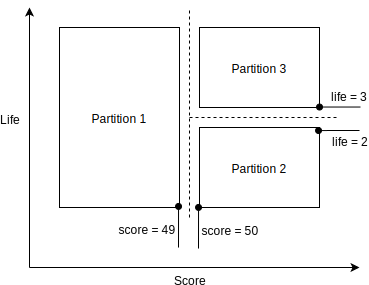
\includegraphics{img/boundary-testing/examples/partition_boundaries.svg}
\caption{Partitions with their boundaries}
\end{figure}

In our example, the tester would then devise and automate test cases B1
and B2. Given that a boundary is composed of two different input values,
note that each boundary will require \emph{at least} two test cases:

For B1: * B1.1 = input=\{score=49, remaining lives=5\}, output=\{99\} *
B1.2 = input=\{score=50, remaining lives=5\}, output=\{150\}

For B2: * B2.1 = input=\{score 500, remaining lives=3\}, output=\{1500\}
* B2.2 = input=\{score 500, remaining lives=2\}, output=\{530\}

An implementation using JUnit is shown below. Note that we have written
just a single test for each pair of test cases. This makes the test more
cohesive. If there is a boundary bug, a single test will let us know.

\begin{Shaded}
\begin{Highlighting}[]
\AttributeTok{@Test}
\DataTypeTok{void} \FunctionTok{betweenLessAndManyPoints}\NormalTok{() \{}
  \FunctionTok{assertEquals}\NormalTok{(}\DecValTok{49}\NormalTok{+}\DecValTok{50}\NormalTok{, pp.}\FunctionTok{totalPoints}\NormalTok{(}\DecValTok{49}\NormalTok{, }\DecValTok{5}\NormalTok{));}
  \FunctionTok{assertEquals}\NormalTok{(}\DecValTok{50}\NormalTok{*}\DecValTok{3}\NormalTok{, pp.}\FunctionTok{totalPoints}\NormalTok{(}\DecValTok{50}\NormalTok{, }\DecValTok{5}\NormalTok{));}
\NormalTok{\}}

\AttributeTok{@Test}
\DataTypeTok{void} \FunctionTok{betweenLessAndManyLives}\NormalTok{() \{}
  \FunctionTok{assertEquals}\NormalTok{(}\DecValTok{500}\NormalTok{*}\DecValTok{3}\NormalTok{, pp.}\FunctionTok{totalPoints}\NormalTok{(}\DecValTok{500}\NormalTok{, }\DecValTok{3}\NormalTok{));}
  \FunctionTok{assertEquals}\NormalTok{(}\DecValTok{500}\NormalTok{+}\DecValTok{30}\NormalTok{, pp.}\FunctionTok{totalPoints}\NormalTok{(}\DecValTok{500}\NormalTok{, }\DecValTok{2}\NormalTok{));}
\NormalTok{\}}
\end{Highlighting}
\end{Shaded}

\{\% hint style=`tip' \%\}

You might have noticed that, for B1, in case of score \textless{} 50,
\texttt{remaining\ lives} makes no difference. However, for score
\textgreater= 50, \texttt{remaining\ lives} does make a difference, as
the output can vary according to its value. And for the B1.2 test case,
we chose \texttt{remaining\ lives} = 5, which makes the condition true.
You might be wondering whether you also need to devise another test
case, B1.3, where the remaining lives condition would be exercised as
false.

If you are looking to test all possible combinations, then the answer is
yes. However, in longer conditions, full of boundaries, the number of
combinations might be too high, making it unfeasible for the developer
to test them all. Later in this chapter, we will learn how to choose
values for the ``boundaries that we do not care about''.

\{\% endhint \%\}

\hypertarget{on-and-off-points}{%
\subsection{On and off points}\label{on-and-off-points}}

Given some initial intuition on how to analyse boundaries, let us define
some terminology:

\begin{itemize}
\tightlist
\item
  \textbf{On-point:} The on-point is the value that is exactly on the
  boundary. This is the value we see in the condition itself.
\item
  \textbf{Off-point}: The off-point is the value that is closest to the
  boundary and that flips the condition. If the on-point makes the
  condition true, the off point makes it false and vice versa. Note that
  when dealing with equalities or inequalities (e.g.~\[x = 6\] or
  \[x \neq 6\]), there are two off-points; one in each direction.
\item
  \textbf{In-points}: In-points are all the values that make the
  condition true.
\item
  \textbf{Out-points}: Out-points are all the values that make the
  condition false.
\end{itemize}

\textbf{Example:} Suppose we have a program that adds shipping costs
when the total price is below 100. The condition used in the program is
\[x < 100\].

\begin{itemize}
\tightlist
\item
  The on-point is \[100\], as that is the value that is precisely in the
  condition.
\item
  The on-point makes the condition false (100 is not smaller than 100),
  so the off-point should be the closest number that makes the condition
  true. This will be \[99\], as \[99 < 100\] is true.
\item
  The in-points are the values which are smaller than or equal to
  \[99\]. For example, 37, 42, 56.
\item
  The out-points are all values which are larger than or equal to
  \[100\]. For example, 325, 1254, 101.
\end{itemize}

We show all these points in the diagram below.

\begin{figure}
\centering
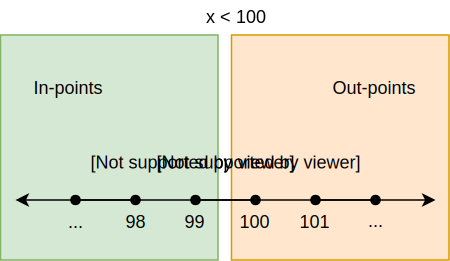
\includegraphics{img/boundary-testing/examples/on_off_points.svg}
\caption{On- and off-points, in- and out-points}
\end{figure}

Let us now study a similar but slightly different condition:
\[x \leq 100\] (the only difference is that, in this one, we use ``less
than or equal to''):

\begin{itemize}
\tightlist
\item
  The on-point is still \[100\]: this is the value that is precisely in
  the condition.
\item
  The condition is evaluated as true for the on-point. So, the off-point
  should be the closest number to the on-point, but making the condition
  false. The off-point is thus \[101\].
\end{itemize}

\begin{figure}
\centering
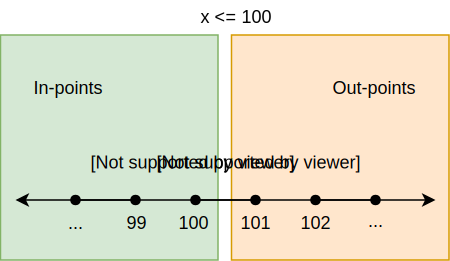
\includegraphics{img/boundary-testing/examples/on_off_points2.svg}
\caption{On-, off-, in- and out-points 2}
\end{figure}

Note that, depending on the condition, an on-point can be either an in-
or an out-point.

As a tester, you devise test cases for these different points: a test
case for the on-point, a test case for the off-point, a test case for a
single in-point (as all in-points belong to the same equivalence
partition), and a test case for a single out-point (as all out-points
also belong to the same equivalence partition).

\{\% hint style=`tip' \%\} Note that \emph{on} and \emph{off} points are
also \emph{in} or \emph{out points}. Therefore, tests that focus only on
the \emph{on} and \emph{off} points would also be testing \emph{in} and
\emph{out} points. In fact, some authors argue that testing boundaries
is enough. Moreover, a test that exercises an in-point that is far away
from the boundary might not have a strong fault detection capability.
Why would we need them?

There is \emph{no perfect answer} here. We suggest:

\begin{itemize}
\tightlist
\item
  If the number of test cases is indeed too high, and it is just too
  expensive to do them all, prioritization is important, and we suggest
  testers to indeed \textbf{focus on the boundaries}.
\item
  Far away in/out points are sometimes easier to be seen or comprehended
  by a tester who is still learning about the system under test, and
  exploring its boundaries (\emph{exploratory testing}). Deciding
  whether to perform such a test is thus a decision that a tester should
  take, taking the costs into account. \{\% endhint \%\}
\end{itemize}

\hypertarget{revisiting-the-chocolate-bars-problem}{%
\subsection{Revisiting the ``chocolate bars''
problem}\label{revisiting-the-chocolate-bars-problem}}

Let's revisit the example from the a previous chapter. There, we had a
program where the goal was to return the number of bars needed in order
to build some boxes of chocolates:

\begin{quote}
\textbf{Chocolate bars}

A package should store a total number of kilos. There are small bars (1
kilo each) and big bars (5 kilos each). We should calculate the number
of small bars to use, assuming we always use big bars before small bars.
Return -1 if it can't be done.

The input of the program is thus the number of small bars, the number of
big bars, and the total number of kilos to store.
\end{quote}

And these were the classes we derived after applying the
category/partition method:

\begin{itemize}
\tightlist
\item
  \textbf{Need only small bars}. A solution that only uses the provided
  small bars.
\item
  \textbf{Need only big bars}. A solution that only uses the provided
  big bars.
\item
  \textbf{Need small + big bars}. A solution that has to use both small
  and big bars.
\item
  \textbf{Not enough bars}. A case in which it's not possible, because
  there are not enough bars.
\item
  \textbf{Not from the specs}: An exceptional case.
\end{itemize}

As we saw in the previous chapter, the following code passed all the
tests we derived:

\begin{Shaded}
\begin{Highlighting}[]
\KeywordTok{public} \KeywordTok{class}\NormalTok{ ChocolateBars \{}
    \KeywordTok{public} \DataTypeTok{static} \DataTypeTok{final} \DataTypeTok{int}\NormalTok{ CANNOT\_PACK\_BAG = {-}}\DecValTok{1}\NormalTok{;}

    \KeywordTok{public} \DataTypeTok{int} \FunctionTok{calculate}\NormalTok{(}\DataTypeTok{int}\NormalTok{ small, }\DataTypeTok{int}\NormalTok{ big, }\DataTypeTok{int}\NormalTok{ total) \{}
        \DataTypeTok{int}\NormalTok{ maxBigBoxes = total / }\DecValTok{5}\NormalTok{;}
        \DataTypeTok{int}\NormalTok{ bigBoxesWeCanUse = }\BuiltInTok{Math}\NormalTok{.}\FunctionTok{min}\NormalTok{(maxBigBoxes, big);}
\NormalTok{        total {-}= (bigBoxesWeCanUse * }\DecValTok{5}\NormalTok{);}

        \KeywordTok{if}\NormalTok{(small \textless{}= total)}
            \KeywordTok{return}\NormalTok{ CANNOT\_PACK\_BAG;}
        \KeywordTok{return}\NormalTok{ total;}
\NormalTok{    \}}
\NormalTok{\}}
\end{Highlighting}
\end{Shaded}

However, the following input makes the program to fail:
\texttt{(2,3,17)}!

package book.ch12;

public class ChocolateBars {

    public static final int CANNOT_PACK_BAG = -1;

    public int calculate(int small, int big, int total) {
        int maxBigBoxes = total / 5;
        int bigBoxesWeCanUse = Math.min(maxBigBoxes, big);
        total -= (bigBoxesWeCanUse * 5);

        if(small < total)
            return CANNOT_PACK_BAG;
        return total;

    }
}


\begin{Shaded}
\begin{Highlighting}[]
\KeywordTok{public} \KeywordTok{class}\NormalTok{ ChocolateBars \{}
    \KeywordTok{public} \DataTypeTok{static} \DataTypeTok{final} \DataTypeTok{int}\NormalTok{ CANNOT\_PACK\_BAG = {-}}\DecValTok{1}\NormalTok{;}

    \KeywordTok{public} \DataTypeTok{int} \FunctionTok{calculate}\NormalTok{(}\DataTypeTok{int}\NormalTok{ small, }\DataTypeTok{int}\NormalTok{ big, }\DataTypeTok{int}\NormalTok{ total) \{}
        \DataTypeTok{int}\NormalTok{ maxBigBoxes = total / }\DecValTok{5}\NormalTok{;}
        \DataTypeTok{int}\NormalTok{ bigBoxesWeCanUse = }\BuiltInTok{Math}\NormalTok{.}\FunctionTok{min}\NormalTok{(maxBigBoxes, big);}
\NormalTok{        total {-}= (bigBoxesWeCanUse * }\DecValTok{5}\NormalTok{);}

        \CommentTok{// we fixed the bug here!}
        \KeywordTok{if}\NormalTok{(small \textless{} total)}
            \KeywordTok{return}\NormalTok{ CANNOT\_PACK\_BAG;}
        \KeywordTok{return}\NormalTok{ total;}
\NormalTok{    \}}
\NormalTok{\}}
\end{Highlighting}
\end{Shaded}

This bug is clearly an instance of a bug that should have been detected
by boundary testing. The problem is that this boundary is just less
explicit from the requirements.

As we defined at the beginning of this chapter, boundaries also happen
when we are going from ``one partition'' to another. There is a ``single
condition'' that we can use as clear source. In these cases, what we
should do is to devise test cases for a sequence of inputs that move
from one partition to another.

\begin{figure}
\centering
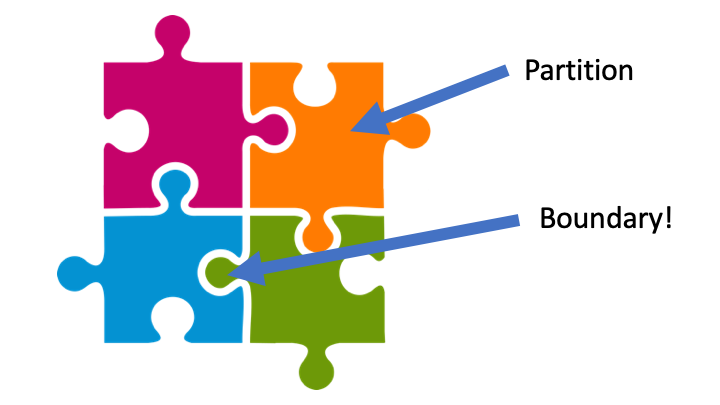
\includegraphics{img/boundary-testing/partition-boundary.png}
\caption{Partitions and boundaries}
\end{figure}

Let us focus on the bug caused by the \texttt{(2,3,17)} input:

\begin{itemize}
\tightlist
\item
  \texttt{(1,3,17)} should return \emph{not possible} (1 small bar is
  not enough). This test case belongs to the \textbf{not enough bars}
  partition.
\item
  \texttt{(2,3,17)} should return 2. This test case belongs to
  \textbf{need for small + big bars} partition.
\end{itemize}

The \texttt{(1,3,17)} and \texttt{(2,3,17)} inputs exercise precisely
the boundary between the \textbf{not enough bars} and the \textbf{need
for small + big bars} partitions.

Let us now explore the boundaries between other partitions. The figure
below shows which boundaries can happen (and that we should test):

\begin{figure}
\centering
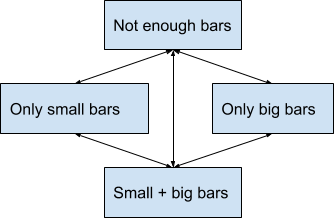
\includegraphics{img/boundary-testing/chocolate-boundaries.png}
\caption{Boundaries in the chocolate bars problem}
\end{figure}

Looking at the \textbf{only big bars} partition, we should find inputs
that transition from this partition to another one:

\begin{itemize}
\tightlist
\item
  \texttt{(10,\ 1,\ 10)} returns 5. This input belongs to the
  \textbf{need small + big bars} partition.
\item
  \texttt{(10,\ 2,\ 10)} returns 0. This input belongs to the
  \textbf{need only big bars} partition.
\end{itemize}

Finally, with the \textbf{only small bars} partition:

\begin{itemize}
\tightlist
\item
  \texttt{(3,\ 2,\ 3)} returns 3. We need only small bars here, and
  therefore, this input belongs to the \textbf{only small bars}
  partition.
\item
  \texttt{(2,\ 2,\ 3)} returns -1. We can't make the boxes. This input
  belongs to the \textbf{Not enough bars} partition.
\end{itemize}

A partition might have boundaries with more than just a single other
partition. The \textbf{only small bars} partition has boundaries not
only with the \textbf{not enough bars} partition (as we saw above), but
also with the \textbf{only big bars} partition:

\begin{itemize}
\tightlist
\item
  \texttt{(4,\ 2,\ 4)} returns 4. We need only small bars here, and
  therefore, this input belongs to the \textbf{only small bars}
  partition.
\item
  \texttt{(4,\ 2,\ 5)} returns 0. We need only big bars here, and
  therefore, this input belongs to the \textbf{only big bars} partition.
\end{itemize}

A lesson we learn from this example is that boundary bugs may not only
emerge out of ``clear \texttt{if} conditions'' we see in the
implementation. Boundary bugs also happen in more subtle interactions
among partitions.

\{\% set video\_id = ``uP\_SpXtHxoQ'' \%\} \{\% include
``/includes/youtube.md'' \%\}

\hypertarget{automating-boundary-testing-with-junit-via-parameterised-tests}{%
\subsection{Automating boundary testing with JUnit (via parameterised
tests)}\label{automating-boundary-testing-with-junit-via-parameterised-tests}}

You might have noticed that in the domain matrix we always have a
certain number of input values and, implicitly, an expected output
value. We could just implement the boundary tests by making a separate
method for each test, or by grouping them per boundary, as we have been
doing so far.

However, the number of test methods can quickly become large and
unmanageable. Moreover, the code in these test methods will be largely
the same, as they all have the same structure, only with different input
and output values.

Luckily, JUnit offers a solution where we can generalise the
implementation of a test method, and run it with different inputs and
expected outputs: \textbf{parameterised Tests}. As the name suggests,
with a parameterised test, developers can define a test method with
parameters. To define a parameterised test, you make use of the
\texttt{@ParameterizedTest} annotation, instead of the usual
\texttt{@Test} annotation.

For each parameter you want to pass to the ``template test method'', you
define a parameter in the method's parameter list (note that so far, all
our JUnit methods had no parameters). For example, a test method
\texttt{t1(int\ a,\ int\ b)} receives two parameters, \texttt{int\ a}
and \texttt{int\ b}. The developer uses these two variables in the body
of the test method, often in places where the developer would have a
hard-coded value.

The next step is to feed JUnit with a list of inputs which will be
passed to the test method. In general, these values are provided by a
\texttt{Source}. Here, we will make use of a \texttt{CsvSource}. With
it, each test case is given as a comma-separated list of input values.
To execute multiple tests with the same test method, the
\texttt{CsvSource} expects list of strings, where each string represents
the input and output values for one test case. The \texttt{CsvSource} is
an annotation itself, so in an implementation it would look like the
following:
\texttt{@CsvSource(\{"value11,\ value12",\ "value21,\ value22",\ "value31,\ value32",\ ...\})}

\begin{Shaded}
\begin{Highlighting}[]
\AttributeTok{@ParameterizedTest}\NormalTok{(name = }\StringTok{"small=\{0\}, big=\{1\}, total=\{2\}, result=\{3\}"}\NormalTok{)}
    \AttributeTok{@CsvSource}\NormalTok{(\{}
      \CommentTok{// The total is higher than the amount of small and big bars.}
      \StringTok{"1,1,5,0"}\NormalTok{, }\StringTok{"1,1,6,1"}\NormalTok{, }\StringTok{"1,1,7,{-}1"}\NormalTok{, }\StringTok{"1,1,8,{-}1"}\NormalTok{,}
      \CommentTok{// No need for small bars.}
      \StringTok{"4,0,10,{-}1"}\NormalTok{, }\StringTok{"4,1,10,{-}1"}\NormalTok{, }\StringTok{"5,2,10,0"}\NormalTok{, }\StringTok{"5,3,10,0"}\NormalTok{,}
      \CommentTok{// Need for big and small bars.}
      \StringTok{"0,3,17,{-}1"}\NormalTok{, }\StringTok{"1,3,17,{-}1"}\NormalTok{, }\StringTok{"2,3,17,2"}\NormalTok{, }\StringTok{"3,3,17,2"}\NormalTok{,}
      \StringTok{"0,3,12,{-}1"}\NormalTok{, }\StringTok{"1,3,12,{-}1"}\NormalTok{, }\StringTok{"2,3,12,2"}\NormalTok{, }\StringTok{"3,3,12,2"}\NormalTok{,}
      \CommentTok{// Only small bars.}
      \StringTok{"4,2,3,3"}\NormalTok{, }\StringTok{"3,2,3,3"}\NormalTok{, }\StringTok{"2,2,3,{-}1"}\NormalTok{, }\StringTok{"1,2,3,{-}1"}
\NormalTok{    \})}
    \DataTypeTok{void} \FunctionTok{boundaries}\NormalTok{(}\DataTypeTok{int}\NormalTok{ small, }\DataTypeTok{int}\NormalTok{ big, }\DataTypeTok{int}\NormalTok{ total, }\DataTypeTok{int}\NormalTok{ expectedResult) \{}
        \DataTypeTok{int}\NormalTok{ result = }\KeywordTok{new} \FunctionTok{ChocolateBars}\NormalTok{().}\FunctionTok{calculate}\NormalTok{(small, big, total);}
\NormalTok{        Assertions.}\FunctionTok{assertEquals}\NormalTok{(expectedResult, result);}
\NormalTok{    \}}
\end{Highlighting}
\end{Shaded}

Some developers prefer not to pass a list of CSV/strings. For those,
JUnit provides a \texttt{@MethodSource} option, which allows developers
to provide the input for the parameterised test through a method. The
developer simply needs to define a method that returns a
\texttt{Stream\textless{}Arguments\textgreater{}} (and set the name of
this method in the \texttt{@MethodSource} annotation). See the
implementation below:

\begin{Shaded}
\begin{Highlighting}[]
\KeywordTok{public} \KeywordTok{class}\NormalTok{ ChocolateBarsTest \{}

    \AttributeTok{@ParameterizedTest}\NormalTok{(name = }\StringTok{"small=\{0\}, big=\{1\}, total=\{2\}, result=\{3\}"}\NormalTok{)}
    \AttributeTok{@MethodSource}\NormalTok{(}\StringTok{"generator"}\NormalTok{)}
    \DataTypeTok{void} \FunctionTok{boundaries}\NormalTok{(}\DataTypeTok{int}\NormalTok{ small, }\DataTypeTok{int}\NormalTok{ big, }\DataTypeTok{int}\NormalTok{ total, }\DataTypeTok{int}\NormalTok{ expectedResult) \{}
        \DataTypeTok{int}\NormalTok{ result = }\KeywordTok{new} \FunctionTok{ChocolateBars}\NormalTok{().}\FunctionTok{calculate}\NormalTok{(small, big, total);}
\NormalTok{        Assertions.}\FunctionTok{assertEquals}\NormalTok{(expectedResult, result);}
\NormalTok{    \}}

    \KeywordTok{private} \DataTypeTok{static}\NormalTok{ Stream\textless{}Arguments\textgreater{} }\FunctionTok{generator}\NormalTok{() \{}
      \KeywordTok{return}\NormalTok{ Stream.}\FunctionTok{of}\NormalTok{(}
        \CommentTok{// The total is higher than the amount of small and big bars.}
\NormalTok{        Arguments.}\FunctionTok{of}\NormalTok{(}\DecValTok{1}\NormalTok{,}\DecValTok{1}\NormalTok{,}\DecValTok{5}\NormalTok{,}\DecValTok{0}\NormalTok{),}
\NormalTok{        Arguments.}\FunctionTok{of}\NormalTok{(}\DecValTok{1}\NormalTok{,}\DecValTok{1}\NormalTok{,}\DecValTok{6}\NormalTok{,}\DecValTok{1}\NormalTok{),}
\NormalTok{        Arguments.}\FunctionTok{of}\NormalTok{(}\DecValTok{1}\NormalTok{,}\DecValTok{1}\NormalTok{,}\DecValTok{7}\NormalTok{,{-}}\DecValTok{1}\NormalTok{),}
\NormalTok{        Arguments.}\FunctionTok{of}\NormalTok{(}\DecValTok{1}\NormalTok{,}\DecValTok{1}\NormalTok{,}\DecValTok{8}\NormalTok{,{-}}\DecValTok{1}\NormalTok{),}
        \CommentTok{// No need for small bars.}
\NormalTok{        Arguments.}\FunctionTok{of}\NormalTok{(}\DecValTok{4}\NormalTok{,}\DecValTok{0}\NormalTok{,}\DecValTok{10}\NormalTok{,{-}}\DecValTok{1}\NormalTok{),}
\NormalTok{        Arguments.}\FunctionTok{of}\NormalTok{(}\DecValTok{4}\NormalTok{,}\DecValTok{1}\NormalTok{,}\DecValTok{10}\NormalTok{,{-}}\DecValTok{1}\NormalTok{),}
\NormalTok{        Arguments.}\FunctionTok{of}\NormalTok{(}\DecValTok{5}\NormalTok{,}\DecValTok{2}\NormalTok{,}\DecValTok{10}\NormalTok{,}\DecValTok{0}\NormalTok{),}
\NormalTok{        Arguments.}\FunctionTok{of}\NormalTok{(}\DecValTok{5}\NormalTok{,}\DecValTok{3}\NormalTok{,}\DecValTok{10}\NormalTok{,}\DecValTok{0}\NormalTok{),}
        \CommentTok{// Need for big and small bars.}
\NormalTok{        Arguments.}\FunctionTok{of}\NormalTok{(}\DecValTok{0}\NormalTok{,}\DecValTok{3}\NormalTok{,}\DecValTok{17}\NormalTok{,{-}}\DecValTok{1}\NormalTok{),}
\NormalTok{        Arguments.}\FunctionTok{of}\NormalTok{(}\DecValTok{1}\NormalTok{,}\DecValTok{3}\NormalTok{,}\DecValTok{17}\NormalTok{,{-}}\DecValTok{1}\NormalTok{),}
\NormalTok{        Arguments.}\FunctionTok{of}\NormalTok{(}\DecValTok{2}\NormalTok{,}\DecValTok{3}\NormalTok{,}\DecValTok{17}\NormalTok{,}\DecValTok{2}\NormalTok{),}
\NormalTok{        Arguments.}\FunctionTok{of}\NormalTok{(}\DecValTok{3}\NormalTok{,}\DecValTok{3}\NormalTok{,}\DecValTok{17}\NormalTok{,}\DecValTok{2}\NormalTok{),}
\NormalTok{        Arguments.}\FunctionTok{of}\NormalTok{(}\DecValTok{0}\NormalTok{,}\DecValTok{3}\NormalTok{,}\DecValTok{12}\NormalTok{,{-}}\DecValTok{1}\NormalTok{),}
\NormalTok{        Arguments.}\FunctionTok{of}\NormalTok{(}\DecValTok{1}\NormalTok{,}\DecValTok{3}\NormalTok{,}\DecValTok{12}\NormalTok{,{-}}\DecValTok{1}\NormalTok{),}
\NormalTok{        Arguments.}\FunctionTok{of}\NormalTok{(}\DecValTok{2}\NormalTok{,}\DecValTok{3}\NormalTok{,}\DecValTok{12}\NormalTok{,}\DecValTok{2}\NormalTok{),}
\NormalTok{        Arguments.}\FunctionTok{of}\NormalTok{(}\DecValTok{3}\NormalTok{,}\DecValTok{3}\NormalTok{,}\DecValTok{12}\NormalTok{,}\DecValTok{2}\NormalTok{),}
        \CommentTok{// Only small bars.}
\NormalTok{        Arguments.}\FunctionTok{of}\NormalTok{(}\DecValTok{4}\NormalTok{,}\DecValTok{2}\NormalTok{,}\DecValTok{3}\NormalTok{,}\DecValTok{3}\NormalTok{),}
\NormalTok{        Arguments.}\FunctionTok{of}\NormalTok{(}\DecValTok{3}\NormalTok{,}\DecValTok{2}\NormalTok{,}\DecValTok{3}\NormalTok{,}\DecValTok{3}\NormalTok{),}
\NormalTok{        Arguments.}\FunctionTok{of}\NormalTok{(}\DecValTok{2}\NormalTok{,}\DecValTok{2}\NormalTok{,}\DecValTok{3}\NormalTok{,{-}}\DecValTok{1}\NormalTok{),}
\NormalTok{        Arguments.}\FunctionTok{of}\NormalTok{(}\DecValTok{1}\NormalTok{,}\DecValTok{2}\NormalTok{,}\DecValTok{3}\NormalTok{,{-}}\DecValTok{1}\NormalTok{)}
\NormalTok{      );}

\NormalTok{    \}}
\NormalTok{\}}
\end{Highlighting}
\end{Shaded}

You can see all these implementation in our GitHub repository:
https://github.com/sttp-book/code-examples/tree/master/src/test/java/tudelft/chocolate.

\{\% set video\_id = ``fFksNXJJfiE'' \%\} \{\% include
``/includes/youtube.md'' \%\}

\hypertarget{the-correct-way}{%
\subsection{The CORRECT way}\label{the-correct-way}}

The book \emph{Pragmatic Unit Testing in Java 8 with JUnit}, by Langr,
Hunt, and Thomas, has an interesting discussion about boundary
conditions. Authors call it the \textbf{CORRECT} way, as each letter
represents one boundary condition to consider:

\begin{itemize}
\tightlist
\item
  \textbf{Conformance:}

  \begin{itemize}
  \tightlist
  \item
    Many data elements must conform to a specific format. Example:
    e-mail addresses (always name@domain). If you expect an e-mail
    address, and you do not receive one, your software might crash.
  \item
    Required action: Test what happens when your input is not in
    conformance with what is expected.
  \end{itemize}
\item
  \textbf{Ordering:}

  \begin{itemize}
  \tightlist
  \item
    Some inputs might come in a specific order. Imagine a system that
    receives different products to be inserted in a basket. The order of
    the data might influence the output. What happens if the list is
    ordered? Unordered?
  \item
    Required action: Make sure our program works even if the data comes
    in an unordered manner (or return an elegant failure to user,
    avoiding the crash).
  \end{itemize}
\item
  \textbf{Range:}

  \begin{itemize}
  \tightlist
  \item
    Inputs should usually be within a certain range. Example: Age should
    always be greater than 0 and smaller than 125.
  \item
    Required action: Test what happens when we provide inputs that are
    outside of the expected range.
  \end{itemize}
\item
  \textbf{Reference:}

  \begin{itemize}
  \tightlist
  \item
    In OOP systems, objects refer to other objects. Sometimes the
    relationships between the objects are extensive and there may be
    external dependencies. What happens if these dependencies do not
    behave as expected?
  \item
    Required action: When testing a method, consider:

    \begin{itemize}
    \tightlist
    \item
      What it references outside its scope
    \item
      What external dependencies it has
    \item
      Whether it depends on the object being in a certain state
    \item
      Any other conditions that must exist
    \end{itemize}
  \end{itemize}
\item
  \textbf{Existence:}

  \begin{itemize}
  \tightlist
  \item
    Does ``something'' really exist? What if it does not? Imagine you
    query a database, and your database returns an empty result. Will
    our software behave correctly?
  \item
    Required action: Does the system behave correctly when something
    that is expected to exist, does not?
  \end{itemize}
\item
  \textbf{Cardinality:}

  \begin{itemize}
  \tightlist
  \item
    In simple words, our loop performed one step less (or more) than it
    should.
  \item
    Required action: Test loops in different situations, such as when it
    actually performs zero iterations, one iterations, or many. (Loops
    are further discussed in the structural testing chapter).
  \end{itemize}
\item
  \textbf{Time}

  \begin{itemize}
  \tightlist
  \item
    Systems rely on dates and times. What happens if the system receives
    inputs that are not ordered in regards to date and time?
  \item
    Timeouts: Does the system handle timeouts well?
  \item
    Concurrency: Does the system handle concurrency well?
  \end{itemize}
\end{itemize}

\{\% set video\_id = ``oxNEUYqEvzM'' \%\} \{\% include
``/includes/youtube.md'' \%\}

\hypertarget{equivalent-classes-and-boundary-analysis-altogether}{%
\subsection{Equivalent classes and boundary analysis
altogether}\label{equivalent-classes-and-boundary-analysis-altogether}}

We discussed \emph{equivalent class analysis} and \emph{boundary
testing}. In practice, testers combine both, in what they call
\emph{domain testing}.

We suggest the following strategy when applying domain testing, highly
influenced by how Kaner et al.~do:

\begin{enumerate}
\def\labelenumi{\arabic{enumi}.}
\tightlist
\item
  We read the requirement
\item
  We identify the input and output variables in play, together with
  their types, and their ranges.
\item
  We identify the dependencies (or independence) among input variables,
  and how input variables influence the output variable.
\item
  We perform equivalent class analysis (valid and invalid classes).
\item
  We explore the boundaries of these classes.
\item
  We think of a strategy to derive test cases, focusing on minimizing
  the costs while maximizing fault detection capability.
\item
  We generate a set of test cases that should be executed against the
  system under test.
\end{enumerate}

See a series of
\href{/chapters/testing-techniques/domain-testing.html}{domain testing
examples} in our appendix.

\hypertarget{exercises}{%
\subsection{Exercises}\label{exercises}}

\textbf{Exercise 1.} We have the following method.

\begin{Shaded}
\begin{Highlighting}[]
\KeywordTok{public} \BuiltInTok{String} \FunctionTok{sameEnds}\NormalTok{(}\BuiltInTok{String}\NormalTok{ string) \{}
  \DataTypeTok{int}\NormalTok{ length = string.}\FunctionTok{length}\NormalTok{();}
  \DataTypeTok{int}\NormalTok{ half = length / }\DecValTok{2}\NormalTok{;}

  \BuiltInTok{String}\NormalTok{ left = }\StringTok{""}\NormalTok{;}
  \BuiltInTok{String}\NormalTok{ right = }\StringTok{""}\NormalTok{;}

  \DataTypeTok{int}\NormalTok{ size = }\DecValTok{0}\NormalTok{;}
  \KeywordTok{for}\NormalTok{(}\DataTypeTok{int}\NormalTok{ i = }\DecValTok{0}\NormalTok{; i \textless{} half; i++) \{}
\NormalTok{    left += string.}\FunctionTok{charAt}\NormalTok{(i);}
\NormalTok{    right = string.}\FunctionTok{charAt}\NormalTok{(length {-} }\DecValTok{1}\NormalTok{ {-} i) + right;}

    \KeywordTok{if}\NormalTok{ (left.}\FunctionTok{equals}\NormalTok{(right))}
\NormalTok{      size = left.}\FunctionTok{length}\NormalTok{();}
\NormalTok{  \}}

  \KeywordTok{return}\NormalTok{ string.}\FunctionTok{substring}\NormalTok{(}\DecValTok{0}\NormalTok{, size);}
\NormalTok{\}}
\end{Highlighting}
\end{Shaded}

Perform boundary analysis on the condition in the for-loop:
\texttt{i\ \textless{}\ half}, i.e.~what are the on- and off-point and
the in- and out-points? You can give the points in terms of the
variables used in the method.

\textbf{Exercise 2.} Perform boundary analysis on the following
equality: \texttt{x\ ==\ 10}. What are the on- and off-points?

\textbf{Exercise 3.} A game has the following condition:
\texttt{numberOfPoints\ \textless{}=\ 570}. Perform boundary analysis on
the condition. What are the on- and off-point of the condition? Also
give an example for both an in-point and an out-point.

\textbf{Exercise 4.} Regarding \textbf{boundary analysis of
inequalities} (e.g., \texttt{a\ \textless{}\ 10}), which of the
following statements \textbf{is true}?

\begin{enumerate}
\def\labelenumi{\arabic{enumi}.}
\tightlist
\item
  There can only be a single on-point which always makes the condition
  true.
\item
  There can be multiple on-points for a given condition which may or may
  not make the condition true.
\item
  There can only be a single off-point which may or may not make the
  condition false.
\item
  There can be multiple off-points for a given condition which always
  make the condition false.
\end{enumerate}

\textbf{Exercise 5.} A game has the following condition:
\texttt{numberOfPoints\ \textgreater{}\ 1024}. Perform a boundary
analysis.

\textbf{Exercise 6.} Perform boundary analysis on the following
decision: \texttt{n\ \%\ 3\ ==\ 0\ \&\&\ n\ \%\ 5\ ==\ 0}. What are the
on- and off-points?

\textbf{Exercise 7.} Which one of the following statements about the
\textbf{CORRECT} principles is \textbf{true}?

\begin{enumerate}
\def\labelenumi{\arabic{enumi}.}
\tightlist
\item
  We assume that external dependencies are already on the right state
  for the test (REFERENCE).
\item
  We test different methods from the same class in an isolated way in
  order to avoid order issues (TIME).
\item
  Whenever we encounter a loop, we always test whether the program works
  for 0, 1, and 10 iterations (CARDINALITY).
\item
  We always test the behaviour of our program when any expected data
  does not exist (EXISTENCE).
\end{enumerate}

\textbf{Exercise 8.} We have a program called IsCat. It works as
follows: \textgreater{} Given an list of prerequisites, it returns
either the string ``Cat'' or the string ``Doge''. \textgreater{} If the
number of legs is an even number, it has a tail, the number of lives
left is between {[}1, 9{]} inclusive, it has sharp nails and the sounds
it produces is ``miauw'', it is a cat. \textgreater{} In any other case,
it is a doge.

First, do boundary analysis on the inputs. Think of on and off points
for each of the conditions (while picking in points for the others).
Next, appply the category/partition method. What are the minimal and
most suitable partitions?

\begin{Shaded}
\begin{Highlighting}[]
\KeywordTok{public} \KeywordTok{class}\NormalTok{ FelineValidator \{}
    \KeywordTok{public} \DataTypeTok{static} \DataTypeTok{final} \BuiltInTok{String}\NormalTok{ INVALID\_CAT = }\StringTok{"doge"}\NormalTok{;}

    \CommentTok{/**}
     \CommentTok{*}\NormalTok{  This function checks whether a certain animal is a cat}\CommentTok{.}
     \CommentTok{*}\NormalTok{  Given the following prerequisites}\CommentTok{:}
     \CommentTok{*}\NormalTok{    If the number of legs is an even number}\CommentTok{,}
     \CommentTok{*}\NormalTok{    it has a tail}\CommentTok{,}
     \CommentTok{*}\NormalTok{    the number of lives left is between }\CommentTok{[1,} \CommentTok{9]}\NormalTok{ inclusive}\CommentTok{,}
     \CommentTok{*}\NormalTok{    it has sharp nails}\CommentTok{,}\NormalTok{ and}
     \CommentTok{*}\NormalTok{    the sounds it produces is }\CommentTok{"}\NormalTok{miauw}\CommentTok{"} \CommentTok{...}
     \CommentTok{*}\NormalTok{  it is a cat}\CommentTok{.}
     \CommentTok{*}\NormalTok{  In any other case}\CommentTok{,}\NormalTok{ it is a doge}\CommentTok{.}
     \CommentTok{*}
     \CommentTok{*} \AnnotationTok{@param numberOfLegs}
     \CommentTok{*} \AnnotationTok{@param hasTail}
     \CommentTok{*} \AnnotationTok{@param numberOfLives}
     \CommentTok{*} \AnnotationTok{@param hasSharpNails}
     \CommentTok{*} \AnnotationTok{@param sound}
     \CommentTok{*} \AnnotationTok{@return }\NormalTok{String}
     \CommentTok{*/}
    \KeywordTok{public} \BuiltInTok{String} \FunctionTok{isCat}\NormalTok{(}\DataTypeTok{int}\NormalTok{ numberOfLegs, }\DataTypeTok{boolean}\NormalTok{ hasTail, }\DataTypeTok{int}\NormalTok{ numberOfLives, }\DataTypeTok{boolean}\NormalTok{ hasSharpNails, }\BuiltInTok{String}\NormalTok{ sound) \{}
        \KeywordTok{if}\NormalTok{ (!(numberOfLegs \% }\DecValTok{2}\NormalTok{ == }\DecValTok{0}\NormalTok{)) }\KeywordTok{return}\NormalTok{ INVALID\_CAT;}
        \KeywordTok{if}\NormalTok{ (!hasTail) }\KeywordTok{return}\NormalTok{ INVALID\_CAT;}
        \KeywordTok{if}\NormalTok{ (!(numberOfLives \textgreater{}= }\DecValTok{1}\NormalTok{ \&\& numberOfLives \textless{}= }\DecValTok{9}\NormalTok{)) }\KeywordTok{return}\NormalTok{  INVALID\_CAT;}
        \KeywordTok{if}\NormalTok{ (!hasSharpNails) }\KeywordTok{return}\NormalTok{ INVALID\_CAT;}
        \KeywordTok{if}\NormalTok{ (!(sound.}\FunctionTok{matches}\NormalTok{(}\StringTok{"miauw"}\NormalTok{))) }\KeywordTok{return}\NormalTok{ INVALID\_CAT;}

        \KeywordTok{return} \StringTok{"cat"}\NormalTok{;}
\NormalTok{    \}}
\NormalTok{\}}
\end{Highlighting}
\end{Shaded}

\hypertarget{references}{%
\subsection{References}\label{references}}

\begin{itemize}
\item
  Jeng, B., \& Weyuker, E. J. (1994). A simplified domain-testing
  strategy. ACM Transactions on Software Engineering and Methodology
  (TOSEM), 3(3), 254-270.
\item
  Chapter 7 of Pragmatic Unit Testing in Java 8 with Junit. Langr, Hunt,
  and Thomas. Pragmatic Programmers, 2015.
\item
  \begin{itemize}
  \tightlist
  \item
    Kaner, Cem, Sowmya Padmanabhan, and Douglas Hoffman. The Domain
    Testing Workbook. Context Driven Press, 2013.
  \end{itemize}
\item
  \begin{itemize}
  \tightlist
  \item
    Kaner, Cem. What Is a Good Test Case?, 2003. URL:
    http://testingeducation.org/BBST/testdesign/Kaner\_GoodTestCase.pdf
  \end{itemize}
\end{itemize}
